\section{Datenbankmodelle}
Datenbankmodelle entscheiden, wie Daten gespeichert werden und wie sie abgerufen werden. Jedes der folgenden Datenbankmodelle hat einen eigenen sinnvollen Use Case. Keins der Modelle ist schlecht, trotzdem hat sich ein relationales Datenbankmodell heutzutage durchgesetzt.
\subsection{Relationales Datenbankmodell}
\begin{figure}[H]
    \centering
    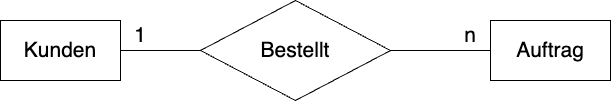
\includegraphics[width=\textwidth]{assets/images/DMRelational}
    \caption{Beispiel Relationales Datenbankmodell}
\end{figure}
Ein relationales Datenbankmodell besteht aus Relationen, dies sind Tabellen. Jede Zeile ist ein Tupel. Ein Tupel ist eine Liste mit fester Länge, welche nicht mehr geändert werden kann. In dem Fall des relationalen Datenbankmodells bestehen die Tupel aus einer Reihe von Attributen. Das Schema einer Relation legt dabei die Anzahl und den Typ der Attribute fest. Ein Datensatz in der Tabelle wird Record genannt.
\begin{procon}
  \pro{Große Verbreitung}
  \pro{Einfach und Flexibel}
  \con{Aufwendige Segmentierung}
  \con{Künstliche Schlüsselattribute wie IDs}
  \con{Anspruchsvolle Komposition}
\end{procon}
\subsection{Hierarchisches Datenbankmodell}
\begin{figure}[H]
    \centering
    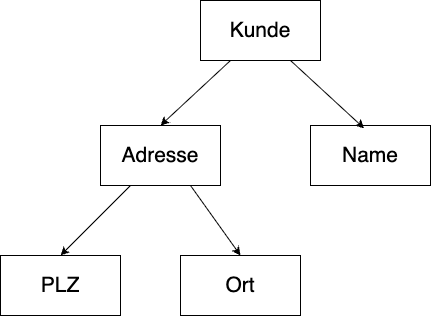
\includegraphics[width=\textwidth]{assets/images/DMHierachie}
    \caption{Beispiel Hierarchisches Datenbankmodell}
\end{figure}
Das hierarchische Modell erinnert an Baumstrukturen. Jede Entität hat einen Vorgänger außer die Erste und kann mehrere Nachfolger haben. Dadurch sind sie gut rekursiv durchsuchbar. Es gibt immer nur einen Einstiegspunkt.
\begin{procon}
\pro{Effiziente computergerechte Datenorganisation}
\pro{Sehr schnell}
\con{Benutzer muss die Datenstruktur gut kennen}
\con{Redundanzen sind möglich}
\end{procon}
\subsection{Netzwerk}
\begin{figure}[H]
    \centering
    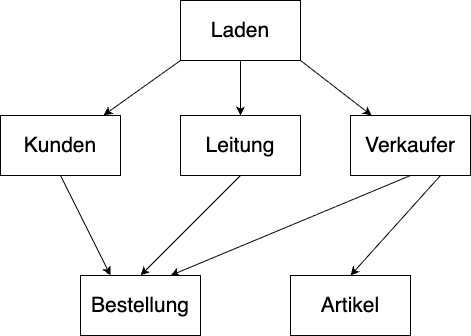
\includegraphics[width=\textwidth]{assets/images/DMNetzwerk}
    \caption{Beispiel Netzwerk Datenbankmodell}
\end{figure}
Das Netzwerkmodell ist nah an dem hierarchischen Modell, allerdings bietet es mehr als einen Einstiegspunkt. So kann man über einen Kunden an dessen Bestellung kommen, aber auch durch den Verkäufer.
\begin{procon}
\pro{Einfache Datenmodellierung, da es keine n-zu-m-Beziehung gibt}
\pro{Komplexe Strukturen können abgebildet werden}
\con{Benutzer muss die Datenstruktur gut kennen}
\con{Unübersichtlich}
\end{procon}
\subsection{Objektorientiert}
\begin{figure}[H]
    \centering
    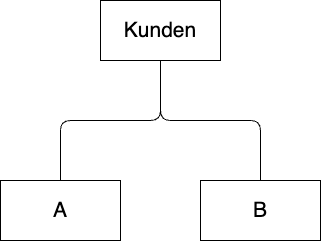
\includegraphics[width=\textwidth]{assets/images/DMObjektorientiert}
    \caption{Beispiel Objektorientiertes Datenbankmodell}
\end{figure}
Bei einem objektorientierten Datenbankmodell werden Objekte ohne Zerlegung gespeichert, also als vollständige Objekte. Auch Vererbung, Kapselung und Polymorphie sind integriert. Dadurch kann man komplexe Datenstrukturen darstellen.

\begin{infobox}
Heutzutage ist das eigentlich obsolet, da es für relationale Datenbanken ORMs gibt, wie z.B. für C\# Entity Framework Core.
\end{infobox}
\begin{procon}
\pro{"Object-relational impedance mismatch" Problem wird behoben}
\pro{Komplexe Kompositionen (JOINS) entfallen}
\pro{Schlüsselverwaltung systemintern}
\con{Bis heute geringe Verbreitung (z.B. db4o), bei Mengenoperationen langsam}
\con{Aufwändige Bearbeitung vererbter Objekte, inkl. Schreibsperren}
\end{procon}
\newpage